\documentclass[a4paper,11pt,notitlepage,fullpage]{article}
%\documentclass{report}

\usepackage{fullpage}
\usepackage[utf8]{inputenc}
%\usepackage[ngerman]{babel}
%\usepackage[english]{babel}
\usepackage{amsmath}
\usepackage{amssymb}
\usepackage{latexsym}
\usepackage{mathtools}
\usepackage{listings}
\usepackage{bbm}
%\usepackage{algorithm}
%\usepackage{algpseudocode}
\usepackage{graphicx}
\usepackage{booktabs}
\usepackage{hhline}
\usepackage{amsthm}
\usepackage{cite}
\usepackage{wrapfig}
\usepackage{hyperref}
\usepackage{titling}
\usepackage{color}

\setlength{\droptitle}{-60pt}

\newcommand{\R}{\mathbb R}
\newcommand{\E}{\mathbb E}
\newcommand{\V}{\mathbb V}
\newcommand{\ind}{\mathbbm{1}}

\begin{document}
\author{Florian Bogner \& Alexander Palmrich}
\title{Stochastische Prozesse - Übung 3}
\maketitle

\begin{enumerate}
\setcounter{enumi}{10}

%11
\item Sei $\eta$ messbar bzgl $\mathcal{F}(a)$ mit $0<a<b$ und $\E[\eta^2]<\infty$.
Es gilt zu zeigen, dass
$$g(t):=\eta \ind_{(a,b]}(t) \in M^2$$
Dafür sollen wir eine Folge $g_n$ in $M^2_\text{step}$ finden, die gegen $g$ geht, im Sinne von
$$\E\left[\int_{\mathbb{R}^+} (g_n-g)^2 dt\right] \stackrel{n\rightarrow\infty}{\rightarrow} 0$$
Wir definieren $g_n := \eta \ind_{[a,b+\frac{1}{n})}(t)$. Das ist eine Folge in $M^2_\text{step}$, weil $\eta$ zum Sprungzeitpunkt $a$ bereits bekannt ist, und weil $\eta$ quadratisch integriebar ist laut Vorraussetzung. Wir rechnen nun nach, dass diese  Folge in der Norm gegen $g$ geht:
\begin{align*}
\left(g_n-g\right)^2 &= \left(\eta \ind_{[a,b+\frac{1}{n})}(t) - \eta \ind_{(a,b]}(t) \right)^2\\
&= \eta^2 \left(\ind_{[a,a]} + \ind_{(b,b+\frac{1}{n})}\right)^2\\
&= \eta^2 \left(\ind_{\{a\}} + \ind_{(b,b+\frac{1}{n})}\right)\\
\Rightarrow \int_{\mathbb{R}^+} \left(g_n-g\right)^2 dt &= \eta^2 \int_{\mathbb{R}^+}\ind_{\{a\}} + \ind_{(b,b+\frac{1}{n})} dt\\
&= \eta^2 \frac{1}{n}\\
\Rightarrow \E \left[\int_{\mathbb{R}^+} \left(g_n-g\right)^2 dt\right] &= \frac{1}{n}\E[\eta^2] \stackrel{n\rightarrow\infty}{\rightarrow} 0
\end{align*}
\hfill $\square$

%12
\item \label{12}Sei $W$ ein Wienerprozess, $0<\alpha <\beta$ fest und
$$f(t):= \ind_{[\alpha, \beta)}(t)$$
Wir sollen das Itō-Integral von $f$ bis zum endlichen Zeitpunkt $t$ bestimmen.
Dazu können wir $f$ als eine "stochastische" Treppenfunktion auffassen und die Definition des Itō-Integrals für Treppenfunktionen bemühen:
\begin{align*}
I_t f &= \int_{\mathbb{R}^+} f(s) \ind_{[0,t)}(s) dW(s)\\
&= \int_{\mathbb{R}^+} \ind_{[\alpha, \beta) \cap [0,t)}(s) dW(s)\\
&= \int_{\mathbb{R}^+} \ind_{[\alpha, t\wedge\beta)}(s) dW(s)\\
&= \int_{\mathbb{R}^+} 1\cdot \ind_{[\alpha, t\wedge\beta)}(s) dW(s)\\
&\hspace{-0.2em}\stackrel{\text{Def}}{=} 1\cdot \left( W(t\wedge\beta) - W(\alpha) \right) \text{ falls } t>\alpha \text{ sonst } 0\\
&= \ind_{(\alpha, \infty)}(t) \left( W(t\wedge\beta) - W(\alpha) \right)
\end{align*}
\hfill $\square$

%13
\item Wir übernehmen Bezeichnungen von Bsp \ref{12}.
\begin{enumerate}
\item Quadratsumme von $f$ über endliche Zeit.
\begin{align*}
\int_0^t f(s)^2 ds &= \int_{\mathbb{R}} \ind_{[0, t)}(s) \ind_{[\alpha, \beta)} (s)^2 ds\\
&= \int_{\mathbb{R}} \ind_{[\alpha, t\wedge\beta)}(s) ds\\
&= t\wedge\beta - \alpha \text{ falls } t>\alpha \text{ sonst } 0\\
&= \left(t\wedge\beta - \alpha\right) \ind_{(\alpha, \infty)}(t)
\end{align*}

\item Varianz von $I_t f$ mittels Itō-Isometrie bestimmen.
$$\V\left[ I_t f\right] = \E\left[ (I_t f)^2 \right] - \E\left[ (I_t f) \right]^2$$
Der erste Term wird mit Isometrie zu dem soeben Ausgerechneten:
\begin{align*}
\E\left[ (I_t f)^2 \right] &= \E\left[ \int f^2 dt \right]\\
&= \E\left[\left(t\wedge\beta - \alpha\right)\ind_{(\alpha, \infty)}(t)\right]\\
&= \left(t\wedge\beta - \alpha\right)\ind_{(\alpha, \infty)}(t)
\end{align*}

Für den zweiten Term verwenden wir die Darstellung aus Bsp \ref{12} und rechnen den Erwartungswert aus:
\begin{align*}
\E\left[ (I_t f) \right]^2 &= \E\left[ \ind_{(\alpha, \infty)}(t) \left( W(t\wedge\beta) - W(\alpha) \right)\right]^2\\
&= \ind_{(\alpha, \infty)}(t) \E\left[ W(t\wedge\beta) - W(\alpha)\right]^2\\
&= \ind_{(\alpha, \infty)}(t) \E\left[ \text{Wiener-Inkrement}\right]^2\\
&= \ind_{(\alpha, \infty)}(t) 0^2\\
&= 0
\end{align*}

Insgesamt erhalten wir also
$$\V\left[ I_t f\right] = \left(t\wedge\beta - \alpha\right)\ind_{(\alpha, \infty)}(t)$$

\item Bedingte Erwartung des Itō-Integrals.
$$\E \left[ I_t f | \mathcal{F}(s)\right] = I_s f$$
falls $s<t$ und $f\in M_t^2$ (was bei uns erfüllt ist), laut der Martingaleigenschaft aus Vorlesung 5. Wir wissen also durch Bsp \ref{12} wie das ausschaut.
\hfill $\square$

\end{enumerate}
%14
\item
\begin{enumerate}
\item $Z = 1_{[1, 2)} W(1) + 1_{[2, 3)} W(2)$ ist eine Treppenfunktion mit 2 Treppen. Man beachte, die vermeintlich erste Treppe ist immer 0, da für $0 \leq t < 1$ gilt $W(\lfloor t\rfloor) = W(0) = 0$.
\begin{figure}[h!]
\centering
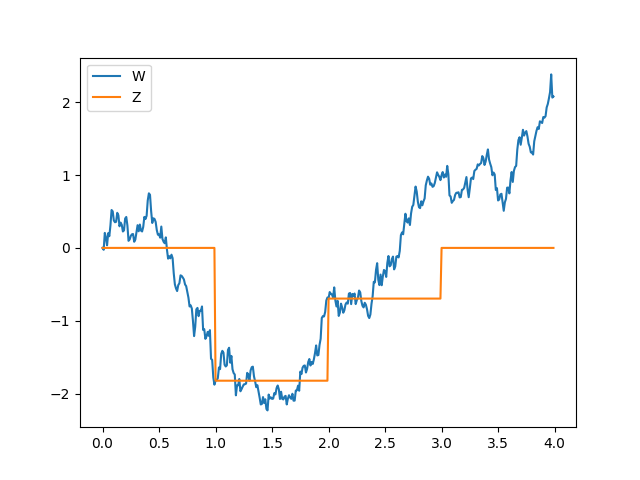
\includegraphics[width=0.66\textwidth]{gfx/14_fig.png}
\caption{Ein typischer Pfad von $W$ und $Z$}
\end{figure}

\item Messbarkeitsbedingung: Der Funktionswert $\eta_j$ muss $\mathcal F(t_j)$-messbar sein, i.e. zu Beginn des Intervalls schon bekannt sein. Dies ist der Fall, da der Funktionswert ja der Wert des Wienerprozesses zu Beginn des Intervalls ist.

Integrabilitätsbedingung: $\infty \stackrel{!}{>} E[\eta_j^2] = E[W(t_j)^2] = V[W(t_j)] = t_j < \infty$

\item Stochastisches Integral für $M_{step}^2$:
\begin{align*}
Y(t) &= \int_0^t Z(s)dW(s) \\
Y(2) &= W(1) \cdot (W(2) - W(1)) \\
Y(3) &= W(1) \cdot (W(2) - W(1)) + W(2) \cdot (W(3) - W(2))
\end{align*}

\item Mit Baby-Itô-Isometrie:
\begin{align*}
E\left[Y(3)^2\right] &= E\left[\int_0^3 Z(s)^2 ~ds\right] \\
&= E\left[\int_0^3 1_{[1, 2)} W(1)^2 + 1_{[2, 3)} W(2)^2 ~ds\right] \\
&= E\left[W(1)^2 + W(2)^2\right] \\
&= 1 + 2 = 3 \\
\end{align*}

\end{enumerate}


%15
\item Angenommen $W$ ist eine Brownsche Bewegung und $f: \R_+ \to \R$ ist eine beschränkte stetige Funktion und $0 \leq t_0 < t_1 < \ldots < t_n$. Welche Verteilung hat die Zufallsvariable
\begin{align*}
U = \sum_{k=1}^n f(t_{k-1})\Delta W(t_k)
\end{align*}
Die vorkommenden Inkremente von $W$ sind bekanntlich unabhängig normalverteilt, i.e. $\Delta W(t_k) \sim N(0, t_k - t_{k-1})$. Demnach ist $U$ eine Linearkombination aus Normalverteilungen und nach dem Reproduktionssatz wieder eine Normalverteilung. Mit
\begin{align*}
A &:= (f(t_0), f(t_1), \ldots, f(t_{n-1}) \in \R^{1\times n} \\
\mu &:= (0, 0, \ldots, 0)^T \in R^n \\
\sigma &:= diag(t_1 - t_0, t_2 - t_1, \ldots, t_n - t_{n-1}) \in \R^{n\times n}
\end{align*}
folgt:
\begin{align*}
U &\sim N\left(A\mu, A^T \sigma A\right) \\
&\sim N\left(0, \sum_{k=1}^n f(t_{k-1})^2(t_k - t_{k-1})\right)
\end{align*}
Erwartungswert und Varianz stehen damit schon da.


\end{enumerate}












\end{document}